\begin{minipage}{0.49\textwidth}
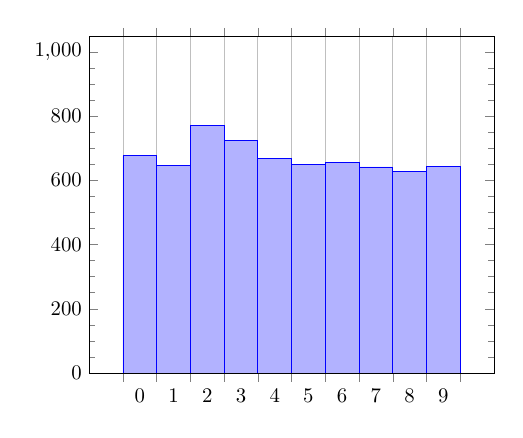
\begin{tikzpicture}[scale=0.75]
  \begin{axis}[ybar interval, ymax=1046.69,ymin=0, minor y tick num = 3]
    \addplot coordinates { (0,676.987) (1,645.972) (2,769.76) (3,723.993) (4,667.89) (5,648.531) (6,656.658) (7,641.198) (8,626.672) (9,641.736) (10, 475.768) };
  \end{axis}
\end{tikzpicture}
\caption*{Average weights repartitions on several trees}
\end{minipage}
\begin{minipage}{0.49\textwidth}
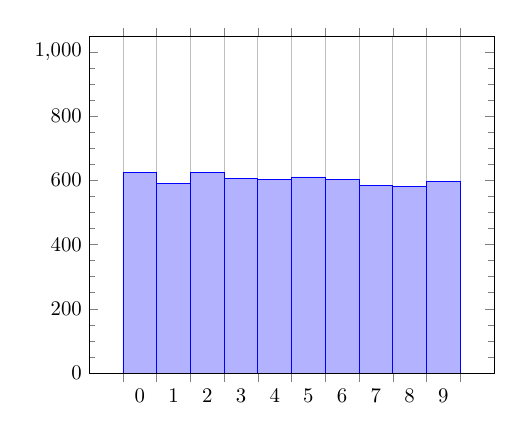
\begin{tikzpicture}[scale=0.75]
  \begin{axis}[ybar interval, ymax=1046.69,ymin=0, minor y tick num = 3]
    \addplot coordinates { (0,624) (1,591.378) (2,625.142) (3,605.63) (4,603.591) (5,610.181) (6,602.677) (7,583.724) (8,581.913) (9,595.063) (10, 475.768) };
  \end{axis}
\end{tikzpicture}
\caption*{Average weights repartitions on one of the trees}
\end{minipage}
\begin{minipage}{0.49\textwidth}
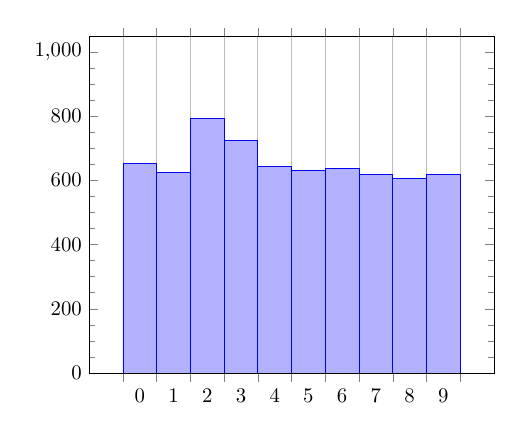
\begin{tikzpicture}[scale=0.75]
  \begin{axis}[ybar interval, ymax=1046.69,ymin=0, minor y tick num = 3]
    \addplot coordinates { (0,652.811) (1,624.504) (2,792.11) (3,724.449) (4,642.961) (5,629.244) (6,637.866) (7,616.693) (8,606.22) (9,619.173) (10, 475.768) };
  \end{axis}
\end{tikzpicture}
\caption*{Average weights repartitions on one of the trees}
\end{minipage}
\begin{minipage}{0.49\textwidth}
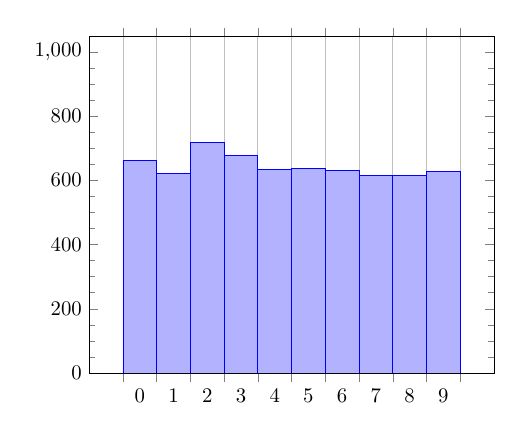
\begin{tikzpicture}[scale=0.75]
  \begin{axis}[ybar interval, ymax=1046.69,ymin=0, minor y tick num = 3]
    \addplot coordinates { (0,662.094) (1,620.48) (2,717.488) (3,676.433) (4,633.465) (5,637.606) (6,631.559) (7,613.992) (8,615.354) (9,628.331) (10, 475.768) };
  \end{axis}
\end{tikzpicture}
\caption*{Average weights repartitions on one of the trees}
\end{minipage}
